% vim: set tw=78 sts=2 sw=2 ts=8 aw et ai:

Virtualization is a concept in which one or more execution environments are simulated through various techniques. These may include hardware and software partitioning, time-sharing, machine emulation and others.\cite{intr-virtualization}

It implies having a machine on which the virtualization takes place, called a \textbf{host machine}, and a firmware or software, called a \textbf{hypervisor} or virtual machine manager, that creates the virtualized or \textbf{guest machine}.

The guest executes its code, but instead of running directly on the underlying hardware, it has to pass through the hypervisor, which may decide to run the instructions on the hardware or modify them beforehand.

\subsection{Hypervisor types}
\label{subsec:hypertypes}

Depending on how they function, there are two types of hypervisors, as classified in \cite{formal-virt}:
\begin{itemize}
\item
\textbf{Type-1} also called \textbf{native} is a hypervisor that runs directly on top of hardware, while the guest machines are run as processes
\item
\textbf{Type-2} is a hypervisor which runs inside an operating system
\end{itemize}

\subsection{Types of virtualization}
\label{subsec:typesvirt}

In order to perform efficient virtualization, most instructions must be executed directly by the hardware. Interpreting the instructions would incur a performance drop\cite{virt-embedded}. 

However, not all instructions can be directly executed. There are two types of such instructions\cite{virt-embedded} :
\begin{itemize}
\item
\textbf{Control-sensitive instructions} which perform changes on hardware resources through various operations, e.g. I/O
\item
\textbf{Behaviour-sensitive instructions} which read the privilege level and might reveal to the guest that it is not running directly on hardware
\end{itemize}

Depending on how the framework handles sensitive instructions, there are two main types of virtualization\cite{vmware}:
\begin{enumerate}
\item
Full virtualization
\item
Paravirtualization
\end{enumerate}

\subsubsection{Full Virtualization}
\label{subsubsec:fullvirt}

This technique is composed of direct execution and binary translation.
As seen in Figure 1, user code is executed directly, while guest OS requests are translated into instructions that modify the virtual hardware.

In this case, the guest OS does not know it is being virtualized. Thus, no modifications to the operating system are necessary. The hypervisor may cache the translated instructions for future use.

\begin{figure}[h!]
\centering
  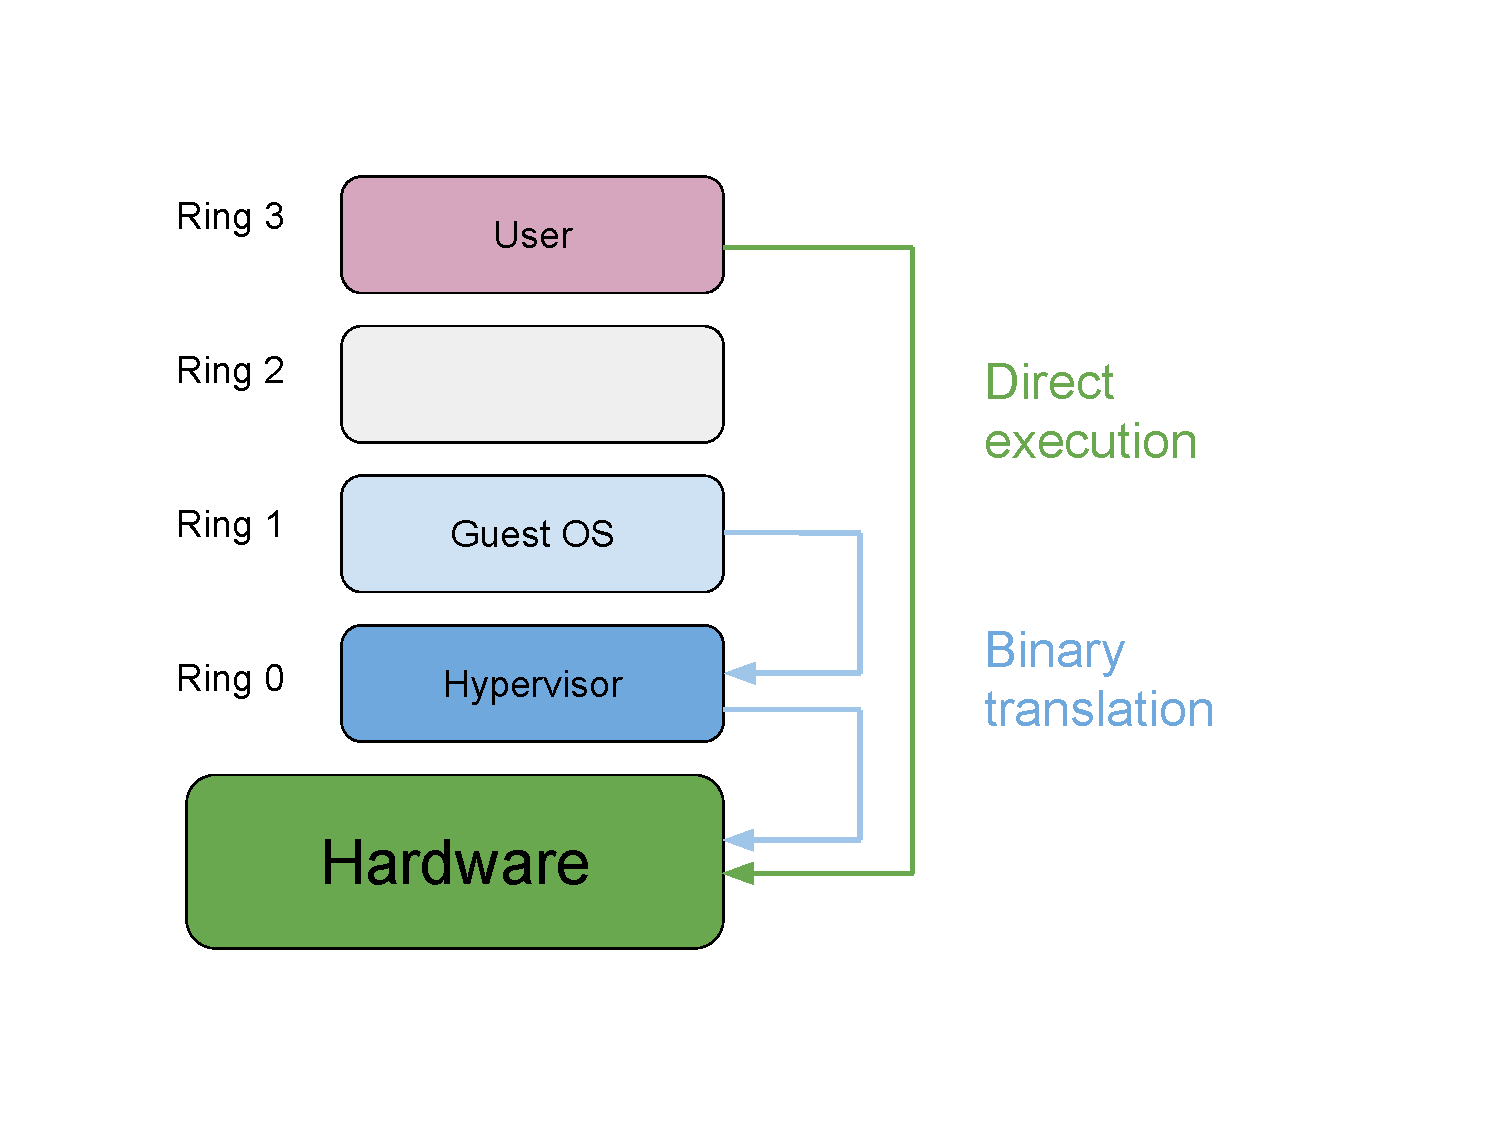
\includegraphics[width=.55\linewidth]{img/fullvirt.pdf}
  \caption{Full Virtualization}
\end{figure}

\subsubsection{Paravirtulization}
\label{subsubsec:paravirt}

Paravirtualization means the hypervisor provides interfaces for operations that are not virtualizable. Because of this, guest OS instructions are now replaced by hypercalls which interact with the virtualization layer.

This approach incurs less performance penalty, but it requires modifications to the operating system which is to be virtualized. In addition, it brings the advantage of being able to replace multiple consecutive sensitive instructions with a single hypercall, reducing the penalty induced by exceptions\cite{virt-embedded}.

\begin{figure}[h!]
\centering
  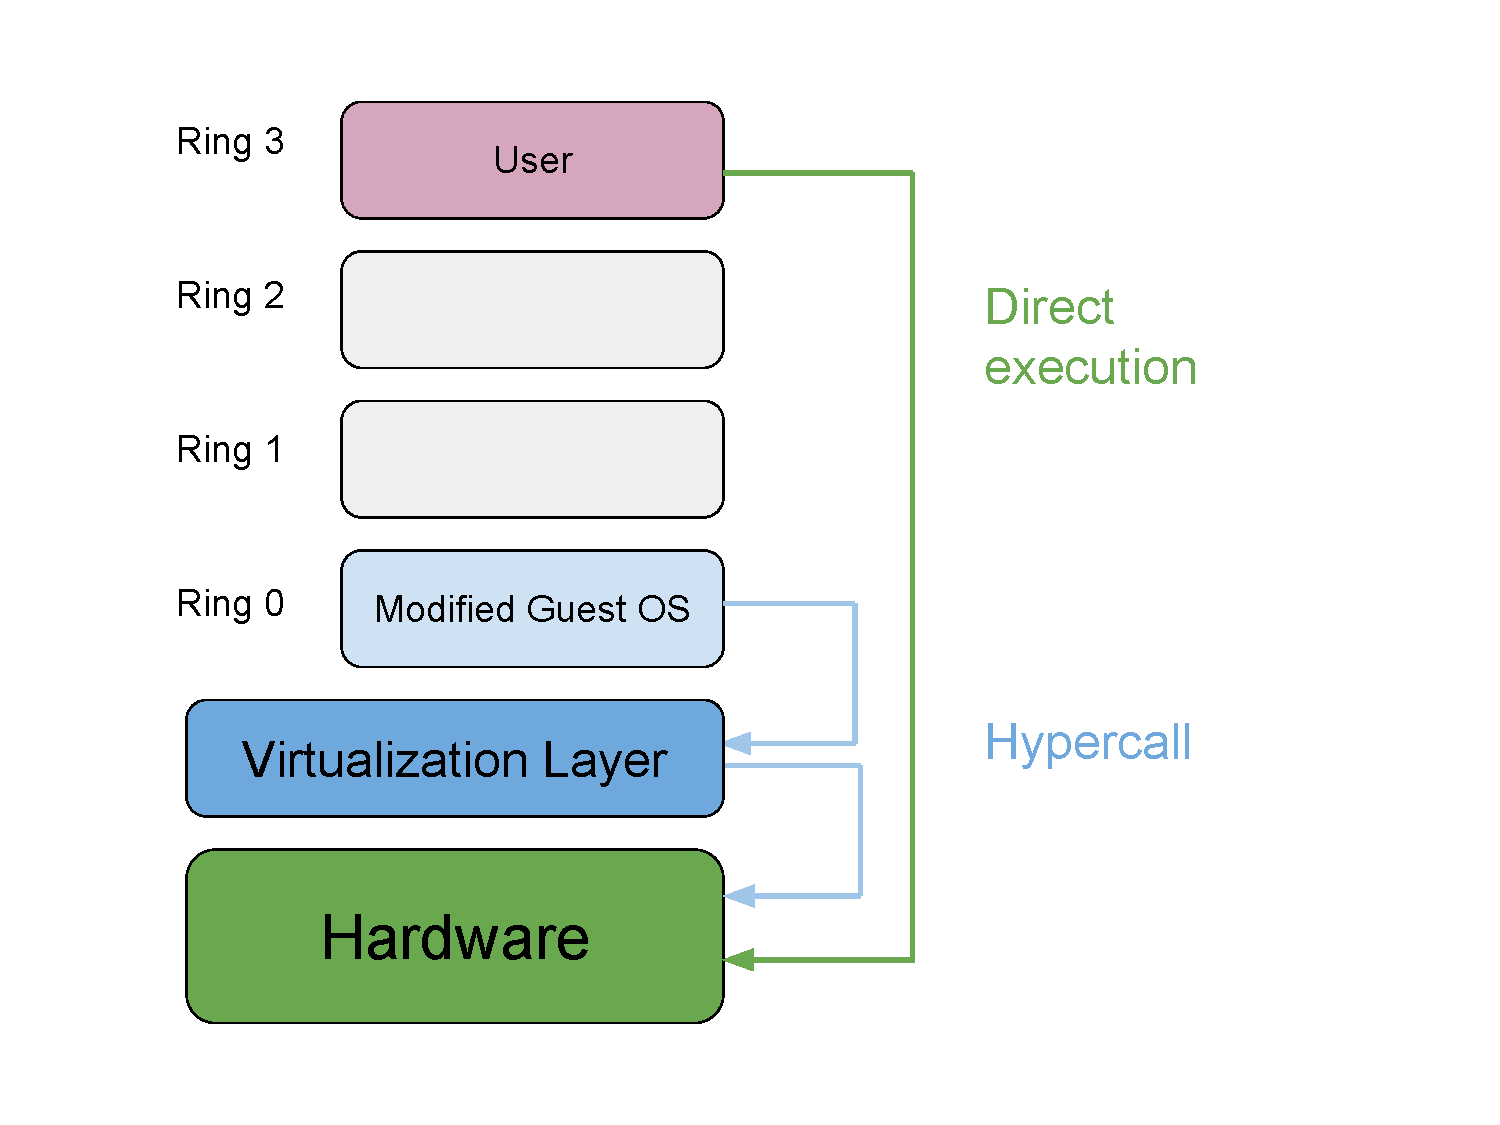
\includegraphics[width=.55\linewidth]{img/paravirt.pdf}
  \caption{Paravirtualization}
\end{figure}

\subsection{Hardware Assisted Virtualization}
\label{subsec:havirt}

In 2006, Intel release its VT-x and AMD presented AMD-V, both introducing the notion of hardware assisted virtualization. The feature consists of a new root level of privilege in which the virtual machine manager runs. Sensitive calls trap to this level without  translation or paravirtualization\cite{vmware}.

Memory is also virtualized in order to accommodate guest systems. This is done by an extra level of indirection in memory management. The memory management unit must map guest physical memory to host machine physical memory\cite{genode-arm}.

\subsection{Virtualization on ARM}
\label{subsec:armvirt}

ARM is a 32-bit RISC architecture. It features one user mode and 6 kernel modes. A secure mode is present, which can be used to protect access to hardware resources and a monitor mode also exists and is responsible for switching between the secure and normal modes\cite{hw-support-arm}.

ARM virtualization works similarly to Intel and AMD, in the sense that it also introduces a new privilege level, namely the \textbf{hyp} mode. In order to handle virtual memory usage while in this mode, an additional memory management unit was introduced. An additional extension, called Large Physical Address Extension, was also added, extending the addressable physical memory space to 40 bits\cite{genode-arm}.

\begin{figure}[h!]
\centering
  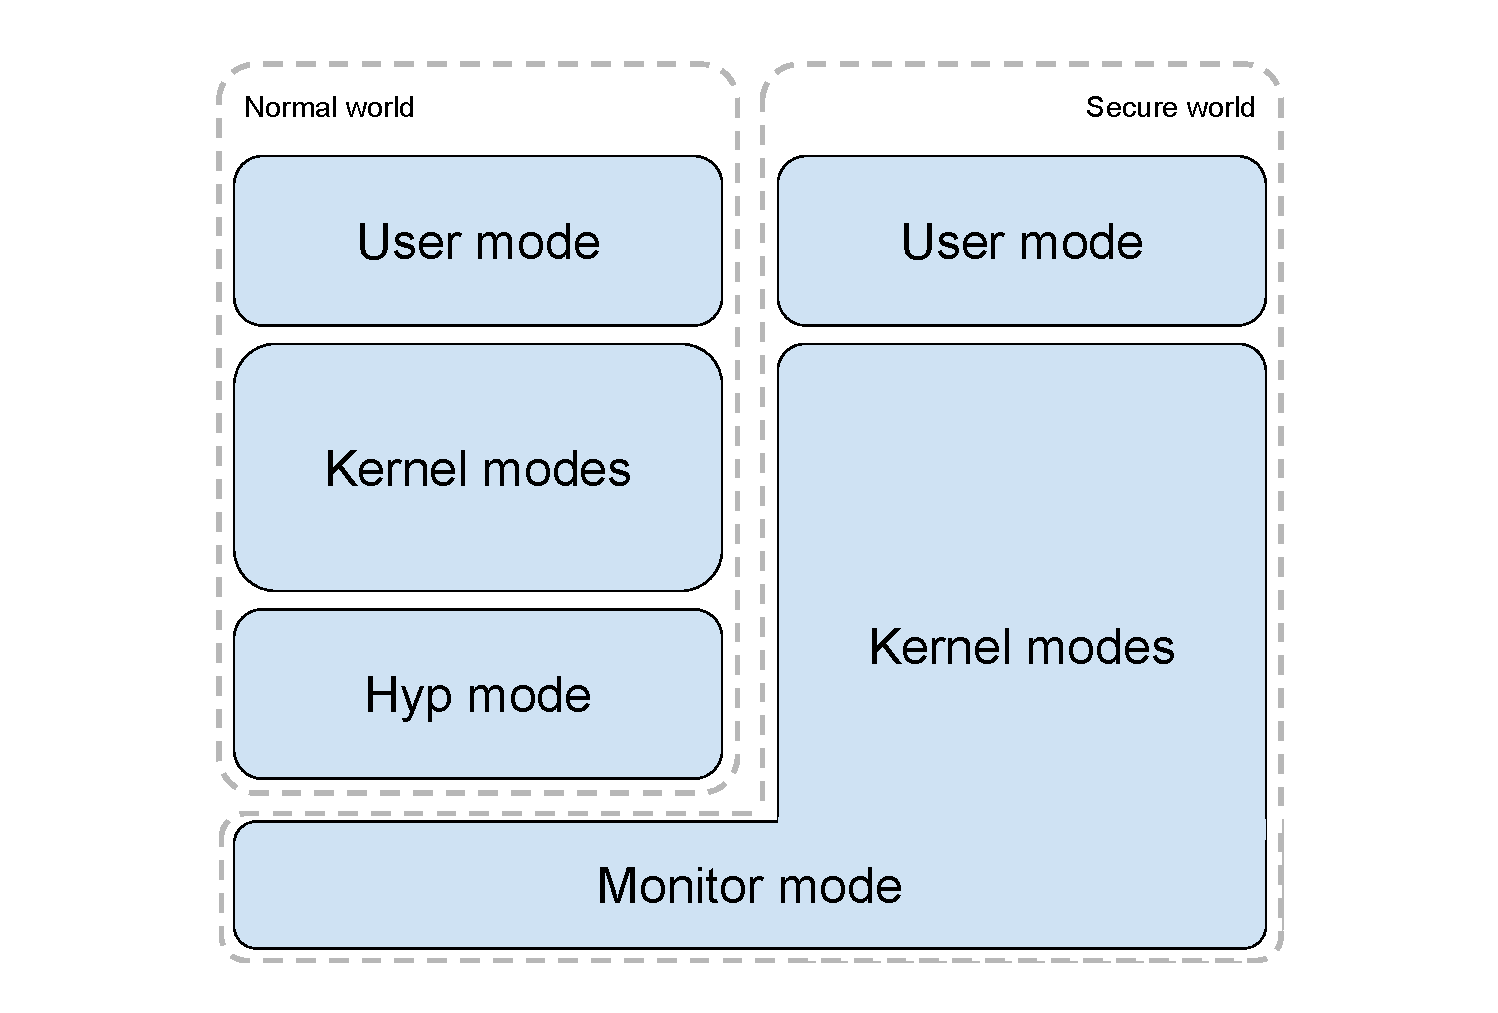
\includegraphics[width=.7\linewidth]{img/arm.pdf}
  \caption{ARM privilege levels}
\end{figure}

Another component introduced by ARM is called \textbf{virtual CPU} which allows virtual interrupts. Such interrupts can either be handled by the hypervisor, or linked directly to the physical interrupt\cite{hw-support-arm}.

\subsection{Advantages of Virtualization for Embedded Systems}
\label{subsec:advvirt}

Advances in performance of embedded systems have made them a viable platform for virtualization. The main reason why virtualization on embedded systems is necessary is to have multiple operating systems, each responsible for some subset of functions performed by the device.

Another important aspect of virtualization is the security benefits it brings. The isolation of one guest from another means that a vulnerability in one subsystem cannot lead to an exploit in another. This limits the possibilities a potential attacker has when trying to compromise a system\cite{virt-embedded}.

The above mentioned isolation also results in the possibility of using software distributed under different license agreements in different guests, while having efficient communication between these facilitated by the hypervisor.

\subsection{Limitations of Virtualization for Embedded Systems}
\label{subsec:limitvirt}

While performance of embedded systems has increased considerably, complexity of software systems has increased as well. The fact that each guest runs a separate operating system renders the virtual machines quite expensive from a resource perspective.

Another issue with performance is brought on by the scheduling mechanism. Due to the encapsulation of virtualized systems, the hypervisor can only associate a priority for each guest system. The result is that a higher priority machine will be preferred while scheduling, regardless of the priority of the task running inside the guest\cite{virt-embedded}.

Although virtualization does bring benefits in terms of security, it has some drawbacks. The increased amount of code on which a guest operating system relies on in order to function equates to increased amount of potential vulnerabilities.
